\documentclass[12pt]{elsarticle}
\usepackage[bottom=2cm,top=3cm,left=3cm,right=2cm]{geometry}
\usepackage{url}
\makeatletter
\def\ps@pprintTitle{%
      	\let\@oddhead\@empty
      	\let\@evenhead\@empty
      	\def\@oddfoot{\reset@font\hfil\thepage\hfil}
      	\let\@evenfoot\@oddfoot
}
\makeatother

\usepackage{babelbib}

\usepackage[brazilian]{babel} % Traduz alguns termos para o português
\usepackage[utf8]{inputenc} % Reconhece acentuação
\usepackage{setspace}

\onehalfspacing

\begin{document}

	\begin{frontmatter}

		\title{ELE083 Computação Evolucionária\\ \resizebox{7cm}{0.3cm}{Trabalho Prático - Makespan}}
		\author{Davi Pinheiro Viana - 2013029912\\Rafael Carneiro de Castro - 2013030210}
		\address{Minas Gerais, Brasil}
		
		\begin{keyword}
			Makespan\sep Computação Evolucionária\sep Evolução Diferencial
		\end{keyword}
	\end{frontmatter}
	
	\section{Introdução}
	O trabalho final da disciplina de Computação Evolucionária consiste no emprego de uma das técnicas estudadas em sala de aula no decorrer do semestre para a solução de um problema de Engenharia. Tal problema é \textit{Job Shop Scheduling Problem} (JSSP).
	
	O \textit{Job Shop Scheduling Problem} é um problema clássico de otimização combinatória e possui diversas aplicações nas indústrias e empresas. Seu objetivo é obter uma sequência de tarefas a serem executadas de forma a maximizar a utilização dos recursos disponíveis. Por recursos, entende-se como máquinas, pessoas, ou ambos.
	
	A nível de contexto, imagina-se uma linha de produção com X etapas, que devem ser executadas em ordem. Tem-se como entrada um arquivo texto contendo Y linhas, que representam Y pedidos, com X números inteiros em cada linha. Estes números representam o tempo que o pedido daquela linha vai gastar em cada etapa. O objetivo é retornar uma sequência de produção dos pedidos em tempo ótimo, de forma que o conjunto de pedidos será entrega o mais rápido possível.
	
	Para este trabalho, considera-se que a linha de produção tem três etapas. Sendo assim, os arquivos de entrada contêm três colunas.

	\section{Desenvolvimento}
	Nesta seção serão apresentadas as decisões tomadas para a implementação de um algoritmo que soluciona o problema descrito na \textit{Introdução}.
	
	\subsection{Representação de Indivíduos}
	Para a decisão da forma de se representar indivíduos, primeiro é importante levar em consideração a entrada do algoritmo. Conforme especificações, a entrada é dada por arquivos textos no formato que pode ser visto na Figura \ref{fig:entrada}. Conforme descrito na \textit{Introdução}, cada linha representa um pedido, e cada coluna representa o tempo gasto em uma etapa de produção (máquina). Os arquivos \textit{entrada\_3.txt}, \textit{entrada\_10.txt} e \textit{entrada\_25.txt} foram disponibilizados junto à especificação deste trabalho.
	\begin{figure}[h]
		\centering
		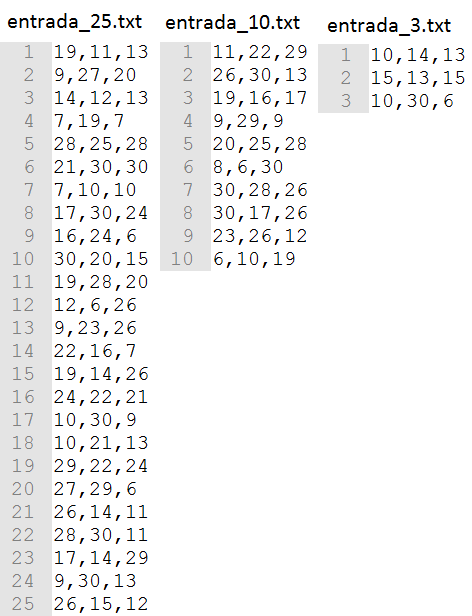
\includegraphics[width=12cm]{img/entrada.png}
		\caption{Exemplos de arquivos de entrada}
		\label{fig:entrada}
	\end{figure}
	
	Em virtude de este ser um problema combinatório cuja saída é uma sequência de produção dos pedidos, os indivíduos podem ser representados por uma sequência de Y números inteiros que vão de 1 até Y, onde Y é a quantidade de pedidos na entrada. Esta sequência é a que otimiza a produção dos pedidos em questão. Sendo assim, as soluções candidatas do problema são representadas por vetores de números inteiros.
	
	\subsection{Algoritmo Evolucionário Escolhido}
	Uma das técnicas e algoritmos estudados em sala de aula foi a chamada \textit{Evolução Diferencial}. Esta é uma técnica amplamente utilizada na solução de problemas através da Computação Evolucionária, possuindo alto desempenho e implementação simples. Sendo assim, esta foi a técnica usada como base para a implementação de uma algoritmo que soluciona o problema em questão neste trabalho.
	
	Conforme visto em sala, um pseudo-código para a \textit{Evolução Diferencial} pode ser observado na Figura \ref{fig:pseudo-code}. No código da figura, é importante se destacar a equação: 
	\[u_{t,i,j} = x_{t,r1,j}+F(x_{t,r2,j}-x_{t,r3,j})\]
	onde $u_{t,i,j}$ representa um indivíduo que sofreu mutação baseado na manipulação vetorial de outros três indivíduos selecionados aleatoriamente. O algoritmo diferencial puro, conforme o representado, é diretamente utilizado para problemas envolvendo otimização contínua. Para problemas combinatórios, como é o caso, adaptações precisam ser feitas, e serão descritas mais a diante.
	\begin{figure}[h]
		\centering
		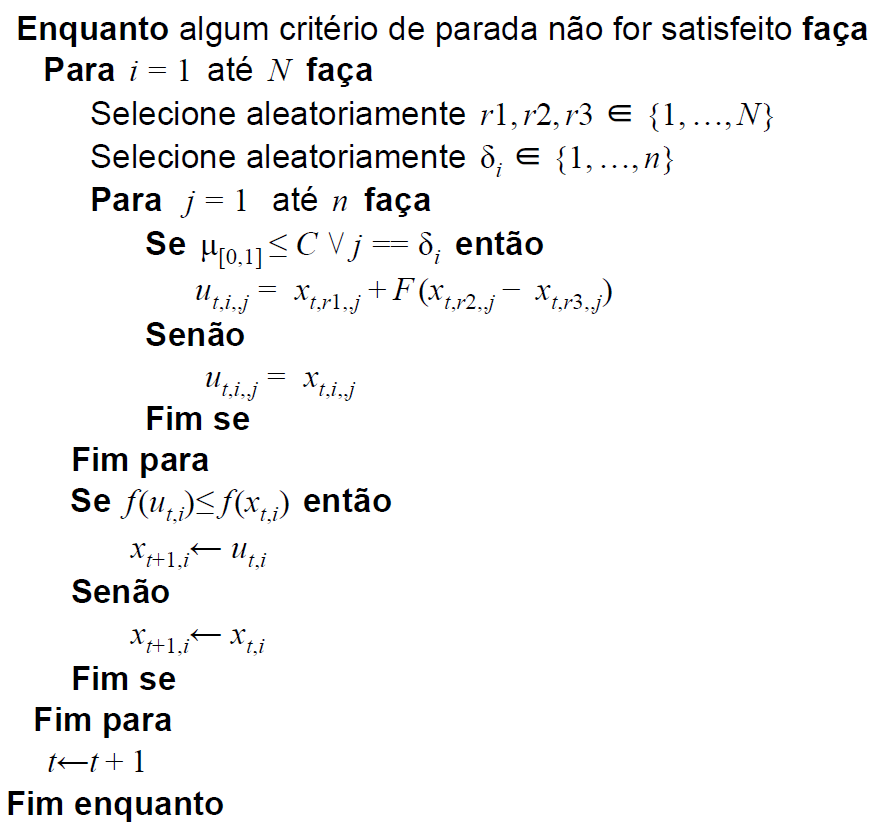
\includegraphics[width=10cm]{img/pseudo-code.png}
		\caption{Pseudo-código para a evolução diferencial}
		\label{fig:pseudo-code}
	\end{figure}
	\pagebreak
	
	\subsection{Operador de Seleção}
	O operador de seleção de sobrevivência do algoritmo de evolução diferencial implementado pode ser visto na condicional \textbf{Se} $f(u_{t,i})<=f(x_{t,i})$ \textbf{então}. Nesta condicional, entende-se por $f(x)$ como a avaliação do \textit{fitness} de um indivíduo. Assim, um indivíduo mutante é selecionado se seu \textit{fitness} é menor que o \textit{fitness} de seu correspondente na população original.
	
	\subsection{Operadores de Cruzamento e Mutação}
	No algoritmo da \textit{Evolução Diferencial}, tanto o cruzamento quanto a mutação podem ser representados pela equação: 
	\[u_{t,i,j} = x_{t,r1,j}+F(x_{t,r2,j}-x_{t,r3,j})\]
	já evidenciada na seção \textit{Algoritmo Evolucionário Escolhido}, junto com a condicional que a cerca, a recombinação discreta. Os parâmetros para tal procedimento são o $C$, representado uma taxa de recombinação, ou seja, uma probabilidade de um indivíduo de uma população mutante ser idêntico a um indivíduo da população original, ou ser um indivíduo mutante de fato; e $F$, que é um fator de escala aplicado ao vetor de diferenças $x_{t,r2,j}-x_{t,r3,j}$.
	
	É importante salientar que a \textit{Evolução Diferencial} seguindo o algoritmo da Figura \ref{fig:pseudo-code} é amplamente utilizada em problemas que envolvem variáveis reais, otimização contínua. Para problemas combinatórios, existem em estudo diversas abordagens e adaptações do mecanismo de cruzamento e mutação. Neste trabalho, optou-se pela abordagem da \textit{Lista de Movimentos}, que é derivada diretamente da equação $u_{t,i,j} = x_{t,r1,j}+F(x_{t,r2,j}-x_{t,r3,j})$. As operações da equação são adaptadas de forma a se encaixar em problemas combinatórios, conforme o descrito a seguir:
	\begin{itemize}
		\item Subtração: como no problema em questão os indivíduos são vetores combinatórios, a subtração é dada por uma lista de movimentos que, se aplicada no primeiro vetor, chega-se ao segundo.
		\item Multiplicação: neste caso, devido ao que foi descrito pela subtração, a multiplicação ocorre entre um escalar e uma lista de movimentos. Assim, defini-se a multiplicação como sendo a seleção de alguns movimentos da lista de movimentos a que se multiplica.
		\item Adição: neste caso, estamos adicionando a um vetor combinatório uma lista de movimentos; ou seja, está-se aplicando a este vetor uma dada quantidade de movimentos.
	\end{itemize}
	
	Como resultado destas operações, tem-se um indivíduo recombinado. Esta técnica é de fácil implementação e possui boa eficiência. Mais detalhes sobre esta e outras abordagens podem ser vistos na Referência [3].
	
	\subsection{Critérios de Parada}
	Como critérios de parada, primeiro estabeleceu-se um número máximo de de gerações como sendo 500, número este que pareceu razoável pelo ajuste de parâmetros que será descrito a seguir. Outro critério de parada baseia-se no histórico. %TODO descrever aqui o critério do histórico%
	
	\subsection{Ajustes de Parâmetros}
	Como mencionado na seção \textit{Operadores de Cruzamento e Mutação}, um dos parâmetros do algoritmo é o $C$ que é a chance de um indivíduo na população mutante ser um indivíduo realmente mutante. Pode ser que seja adicionada à população mutante um indivíduo idêntico à população original, dependendo do valor de $C$. Este parâmetro foi ajustado com o valor de $0.8$, fazendo com que a população mutante criada a cada geração tenha uma grande quantidade de indivíduos mutantes, aumentando a abrangência de uma iteração, ou seja, de um teste sobre uma geração, envolvendo população original e população mutante.
	
	O parâmetro $F$, que representa o fator de escala, foi ajustado com o valor $0.9$, de forma a gerar um indivíduo com uma boa quantidade de permutações de valores partindo de um indivíduo base.
	
	Para o tamanho da população, achamos razoável utilizar o quadrado da quantidade de linhas da entrada, ou seja, o quadrado da quantidade de pedidos. Este valor foi utilizado por causa da variabilidade combinada com os outros parâmetros ajustados. É importante ressaltar que o tamanho populacional foi definido pensando que a entrada com maior quantidade de linhas que será passada ao algoritmo possui 25 linhas. Definiu-se como tamanho máximo da população 1000 indivíduos, para casos de entrada com muitos pedidos. Também é importante destacar que cada geração do algoritmo de \textit{Evolução Diferencial} não aumenta o tamanho da população, ou seja, este valor se mantém constante durante a execução do algoritmo.
	
	\subsection{Avaliação do Fitness}
	%TODO fazer uma explicação rápida do fitness%
	
	\section{Referências}
	\begin{enumerate}
		\item Especificação do trabalho
		\item Notas de aula: \textit{Algoritmo de Evolução Diferencial} - CASTRO, Cristiano
		\item \textit{Uma Nova Abordagem Para A Evolução Diferencial Em Otimização Discreta} - PRADO, Ricardo Sérgio. Disponível em http://www.eletrica.ufpr.br/anais/cba/2010/Artigos/65881\_1.pdf
	\end{enumerate}
	
\end{document}